
当C++11中引入右值引用以支持移动语义时,将表达式划分为左值和右值的方法已不足以描述C++11的所有语言行为。因此,C++标准化委员会基于三个核心类别和两个复合类别,重新设计了价值类别系统(参见图B.1)。核心类别是:左值、prvalue(“纯右值”)和xvalue("过期值")。复合类别是:glvalue(“广义左值”,是左值和xvalue的并集)和rvalue (xvalue和prvalue的并集)。

所有表达式仍然是左值或右值,但右值类别现在会进一步细分。

\begin{center}
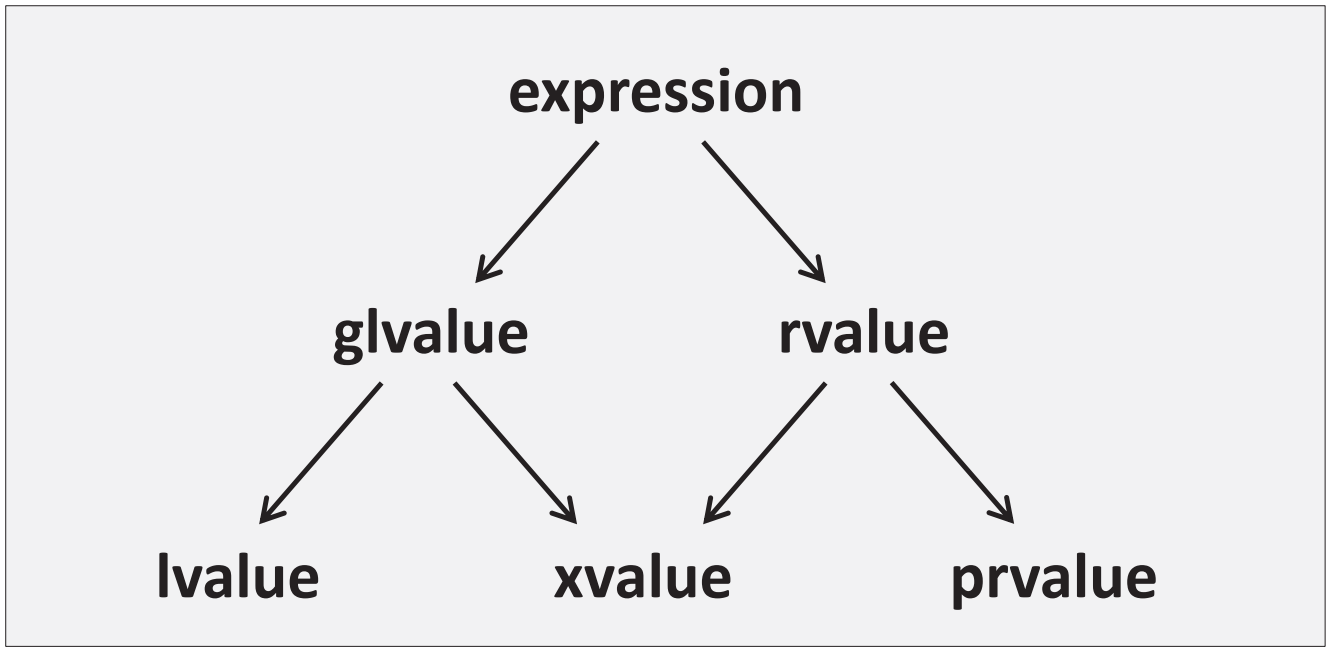
\includegraphics[width=0.8\textwidth]{content/Appendix/B/images/1.png} \\
图B.1. 自C++11后的值类别
\end{center}

C++11的分类在C++17中仍然有效,但C++17的分类重新表述如下:

\begin{itemize}
\item 
glvalue是一个表达式,其计算值决定了对象、位域或函数(即具有存储空间的实体)的标识。

\item 
prvalue是一个表达式,其求值是初始化一个对象或位域,或计算操作符的操作数的值。

\item 
xvalue是glvalue,指定一个对象或位域,其资源可以重用(通常是因为其即将"过期"——xvalue中的"x"最初来自"过期值"(eXpiring value))。

\item 
左值为不是xvalue的glvalue。

\item 
右值为prvalue或xvalue的表达式。
\end{itemize}

C++17中(某种程度上,C++11和C++14也是如此),glvalue和prvalue的区别比传统的左值和右值的区别更为基础。

虽然这描述了在C++17中引入的特性,这些描述也适用于C++11和C++14(之前的描述是相同的,但很难推断)。

除位域外,glvalue生成带有地址的实体。该地址可以是更大的封闭对象子对象的地址。在基类子对象的情况下,glvalue(表达式)类型称为其静态类型,而基类所属的派生对象类型,称为glvalue的动态类型。若glvalue不生成基类子对象,则其静态和动态类型相同(即表达式的类型)。

左值的例子有:

\begin{itemize}
\item 
指定变量或函数的表达式

\item 
内置一元乘法运算符(“指针间接”)的应用

\item 
只是字符串字面量的表达式

\item 
调用返回类型为左值引用的函数
\end{itemize}

prvalue的例子有:

\begin{itemize}
\item 
由非字符串字面量或用户定义字面量的字面量组成的表达式

\begin{notice}用户定义的字面量可以生成左值或右值,这取决于相关字面量操作符的返回类型。
\end{notice}

\item 
内置的一元\&操作符的应用(例如,取表达式的地址)

\item 
内置算术运算符的应用

\item 
对返回类型不是引用类型函数的调用

\item 
Lambda表达式
\end{itemize}

xvalue的例子有:

\begin{itemize}
\item 
调用返回类型为对象类型右值引用的函数(std::move())

\item 
转换为对对象类型的右值引用
\end{itemize}

对函数类型的右值引用会产生左值,而不是xvalue。

需要强调的是,glvalue、prvalue、xvalue等都是表达式,而不是值

\begin{notice}这些术语属于用词不当。
\end{notice}

或实体。例如,变量不是左值,尽管表示该变量的表达式是左值:

\begin{cpp}
int x = 3; // x here is a variable, not an lvalue. 3 is a prvalue initializing
		  // the variable x.
int y = x; // x here is an lvalue. The evaluation of that lvalue expression does not
		  // produce the value 3, but a designation of an object containing the value 3.
		  // That lvalue is then then converted to a prvalue, which is what initializes y.
\end{cpp}

\subsection{B.2.1\hspace{0.2cm}临时实现}

前面提到过,左值通常要进行到右值的转换

\begin{notice}使用C++11的值分类,短语glvalue到prvalue的转换会更准确,但传统术语仍然更为常见。
\end{notice}

因为值是初始化对象(或为大多数内置操作符提供操作数)的表达式类型。

C++17中,这种转换有一个对偶形式,称为临时实现(也可以称为“glvalue到prvalue的转换”):只要期望glvalue(包括xvalue)出现的prvalue有效,就会创建一个临时对象,并使用prvalue初始化(回想一下,prvalue主要是“初始化值”),然后用指定临时的xvalue替换prvalue。例如:

本例中的f()有一个引用参数,所以需要一个glvalue参数。表达式3是一个prvalue,因此“临时实现”规则开始发挥作用。表达式3“转换”为一个xvalue,该xvalue指定一个用值3初始化的临时对象。

在以下情况下,临时对象会实现,并用prvalue进行初始化:

\begin{itemize}
\item 
prvalue绑定到引用(上面调用f(3))。

\item 
访问类prvalue的成员。

\item 
数组prvalue的下标。

\item 
数组prvalue转换为指向其第一个元素的指针(数组衰变)。

\item 
prvalue出现在一个带括号的初始化列表中,对于某些类型X,其初始化std::initializer\_list<X>类型的对象。

\item 
将sizeof或typeid操作符应用于prvalue。

\item 
prvalue是“expr;”形式的语句中的顶层表达式,或者将表达式转换为void。
\end{itemize}

C++17中,由prvalue初始化的对象由上下文决定,因此临时对象只在真正需要时才创建。C++17前,prvalue(特别是类)总是隐含一个临时变量。这些临时变量的副本以后可以有选择地省略,但是编译器仍然需要强制执行复制操作的大多数语义约束(需要复制构造函数可调用)。下面的例子展示了C++17修改规则的结果:

\begin{cpp}
class N {
	public:
	N();
	N(N const&) = delete; // this class is neither copyable ...
	N(N&&) = delete; // ... nor movable
};

N make_N() {
	return N{}; // Always creates a conceptual temporary prior to C++17.
} 				// In C++17, no temporary is created at this point.

auto n = make_N(); // ERROR prior to C++17 because the prvalue needs a
				// conceptual copy. OK since C++17, because n is
				// initialized directly from the prvalue.
\end{cpp}

C++17前,prvalue N\{\}生成了一个类型为N的临时变量,允许编译器删除该临时变量的复制和移动构造(实际上它们总是这样做的)。这意味着调用make\_N()的临时结果可以直接在N的存储中构造,不需要进行复制或移动操作。但C++17前的编译器仍需要检查,是否可以进行复制或移动操作,在本例中这是不可能的,因为N的复制构造函数删除了(并且没有生成移动构造函数)。因此,C++11和C++14编译器必须对这个例子产生错误信息。

C++17中,prvalue N本身不会产生一个临时变量,会初始化了一个由上下文决定的对象:这个对象是N表示的对象。不考虑复制或移动操作(这不是优化,而是语言保证),因此代码是有效的C++17代码。

我们以一个展示各种值类别情况的例子作为结束:

\begin{cpp}
class X {
};

X v;
X const c;

void f(X const&); // accepts an expression of any value category
void f(X&&); // accepts prvalues and xvalues only but is a better match
			// for those than the previous declaration

f(v); // passes a modifiable lvalue to the first f()
f(c); // passes a nonmodifiable lvalue to the first f()
f(X()); // passes a prvalue (since C++17 materialized as xvalue) to the 2nd f()
f(std::move(v)); // passes an xvalue to the second f()
\end{cpp}









